\documentclass{beamer}
\usepackage{amsmath,amsbsy,amsopn,amstext,amsfonts,amssymb}
\usepackage{isomath}
\usepackage{ulem}
%\linespread{1.6}  % double spaces lines
\usepackage{graphicx}
\usepackage{subfigure}
\usepackage{color}
\usepackage{optidef}  % define optimization problems
\usepackage{multicol}  % multiple columns
\usepackage{listings} % for python code
\usepackage{mathrsfs}

\usepackage{polynom}
\newcommand{\adj}{\mathrm{adj}}
\newcommand{\constrainedmin}[3]{
		\begin{mini*}|s|
		{#2}{#1}{}{}
		\addConstraint{#3}
		\end{mini*}
}

\newcommand{\rwbcomment}[1]{{\color{blue}RWB:#1}}
\newcommand{\defeq}{\stackrel{\triangle}{=}}
\newcommand{\abs}[1]{\left|#1\right|}
\newcommand{\norm}[1]{\left\|#1\right\|}
\newcommand{\iprod}[1]{\left<#1\right>}
\newcommand{\ellbf}{\boldsymbol{\ell}}
\newcommand{\nubf}{\boldsymbol{\nu}}
\newcommand{\mubf}{\boldsymbol{\mu}}
\newcommand{\abf}{\mathbf{a}}
\newcommand{\bbf}{\mathbf{b}}
\newcommand{\cbf}{\mathbf{c}}
\newcommand{\dbf}{\mathbf{d}}
\newcommand{\ebf}{\mathbf{e}}
\newcommand{\fbf}{\mathbf{f}}
\newcommand{\gbf}{\mathbf{g}}
\newcommand{\hbf}{\mathbf{h}}
\newcommand{\ibf}{\mathbf{i}}
\newcommand{\jbf}{\mathbf{j}}
\newcommand{\kbf}{\mathbf{k}}
\newcommand{\lbf}{\mathbf{l}}
\newcommand{\mbf}{\mathbf{m}}
\newcommand{\nbf}{\mathbf{n}}
\newcommand{\obf}{\mathbf{o}}
\newcommand{\pbf}{\mathbf{p}}
\newcommand{\qbf}{\mathbf{q}}
\newcommand{\rbf}{\mathbf{r}}
\newcommand{\sbf}{\mathbf{s}}
\newcommand{\tbf}{\mathbf{t}}
\newcommand{\ubf}{\mathbf{u}}
\newcommand{\vbf}{\mathbf{v}}
\newcommand{\wbf}{\mathbf{w}}
\newcommand{\xbf}{\mathbf{x}}
\newcommand{\ybf}{\mathbf{y}}
\newcommand{\zbf}{\mathbf{z}}
\newcommand{\Jbf}{\mathbf{J}}
\newcommand{\Acal}{\mathcal{A}}
\newcommand{\Bcal}{\mathcal{B}}
\newcommand{\Lcal}{\mathcal{L}}
\newcommand{\Ncal}{\mathcal{N}}
\newcommand{\Rcal}{\mathcal{R}}
\definecolor{darkolivegreen}{rgb}{0.33, 0.42, 0.18}

\makeatletter
\newenvironment<>{proofstart}[1][\proofname]{%
    \par
    \def\insertproofname{#1\@addpunct{.}}%
    \usebeamertemplate{proof begin}#2}
  {\usebeamertemplate{proof end}}
\newenvironment<>{proofcont}{%
  \setbeamertemplate{proof begin}{\begin{block}{}}
    \par
    \usebeamertemplate{proof begin}}
  {\usebeamertemplate{proof end}}
\newenvironment<>{proofend}{%
    \par
    \pushQED{\qed}
    \setbeamertemplate{proof begin}{\begin{block}{}}
    \usebeamertemplate{proof begin}}
  {\popQED\usebeamertemplate{proof end}}
\makeatother

\title{ECEn 671: Mathematics of Signals and Systems}
\author{Randal W. Beard}
\institute{Brigham Young University}
\date{\today}

\begin{document}

%-------------------------------
\begin{frame}
	\titlepage
\end{frame}



%%%%%%%%%%%%%%%%%%%%%%%%%%%%%%%%%%%%%%%%%%%%%%%%%%%%%%%%%%%%%%%%%%%%%%%
\section{Topology}
\frame{\sectionpage}

%----------------------------------
\begin{frame}\frametitle{Topology}

\begin{itemize}
\item In this next section, we develop a set of tools that fall under that category of \underline{topology}.  
\item These tools hold for metric spaces (including norm and inner product spaces).
\item WARNING:  There are a lot of definitions.  These definitions will help talk formally about things in the future.
\end{itemize}
\end{frame}

%----------------------------------
\begin{frame}\frametitle{Topology: Open and Closed Sets}

\begin{definition}[Ball] Given a metric space $(\mathbb{X},d)$ a $\delta$-ball around $x_0$ is defined to be
\(
B(x_0,\delta) = \{ x \in \mathbb{X} : d(x,x_0) < \delta \}
\)
\end{definition}
\begin{definition}[Interior Point]
 A point $x_o \in \mathbb{X}$ is interior to $S \subset \mathbb{X}$ if 
\(
\exists \delta > 0 \text{ such that } B(x_o,\delta) \subset S.
\)
\end{definition}
\begin{definition}[Open Set] A set $\mathbb{X}$ is \underline{open} if all points in $\mathbb{X}$ are interior.	
\end{definition}

\begin{definition}[Closed Set] A set $S$ is closed in $\mathbb{X}$ if $\mathbb{X}\setminus S$ is open.	
\end{definition}

\end{frame}

%----------------------------------
\begin{frame}\frametitle{Topology: Convergence}

Let $(\mathbb{X},d)$ be a metric space.

\begin{definition}[Convergence] Given a sequence $\{x_n\}_{n=1}^\infty$, where $x_n\in\mathbb{X}$, the following are equivalent
\begin{itemize}
  \item $\lim_{n \to \infty} x_n = x^*$
  \item $x_n \rightarrow x^*$
  \item $\forall \epsilon > 0, \exists N(\epsilon) \text{ such that } n \geq N \Rightarrow d(x_n,x^*) < \epsilon$
\end{itemize}
A sequence $\{x_n\}_{n=1}^\infty$ in $\mathbb{X}$ with a limit $x^\ast \in \mathbb{X}$ is said to converge.
\end{definition}
\end{frame}

%----------------------------------
\begin{frame}\frametitle{Topology: Convergence}

Note that a limit may not always exist (similar to min, max)
    
    For example, $\lim_{t\to\infty}sin(t)$ does not exist. \\
   
\begin{definition}[$\lim\sup$] Define $\lim \sup$ as the largest limit (possibly infinity) of any subsequence.	
\end{definition}
\begin{definition}[$\lim\inf$]
Define $\lim \inf$ is the smallest limit of all possible subsequences.
\end{definition}

\begin{example}
\begin{itemize}
\item $\underset{t\to\infty}{\lim\sup} \enspace \sin(t) = 1 $ since the subsequence $t_n = \frac{k\pi}{2}, k = 1,5,9,\cdots$ converges to 1
\item $\underset{t\to\infty}{\lim\inf} \enspace \sin(t) = -1 $ since the subsequence $t_n = \frac{k\pi}{2}, k = 3,7,11,\cdots$ converges to -1
\end{itemize}
\end{example}
\end{frame}

%----------------------------------
\begin{frame}\frametitle{Topology: Cauchy Sequence}

\begin{definition}[Cauchy Sequence]
A sequence $\{x_n\}_{n=1}^\infty$ in a metric space $(\mathbb{X},d)$ is said to be a Cauchy sequence if $\forall \epsilon > 0 , \exists N(\epsilon) > 0$ such that $n,m > N \Rightarrow d(x_n,x_m) < \epsilon$
\end{definition}

A sequence is Cauchy if elements in its tail get increasingly closer together.  Note that we have not said anything about an element of convergence.

\begin{theorem} If a sequence $\{x_n\}_{n=1}^\infty$ in $\mathbb{X}$ converges to an element $x^\ast\in\mathbb{X}$ then it is a Cauchy sequence.  	
\end{theorem}


The converse is not true!!  I.e., not all Cauchy sequences converge.  
\end{frame}


%----------------------------------
\begin{frame}\frametitle{Topology: Cauchy Sequence}

\begin{example}[from book]
Let $\mathbb{X} = C[-1,1]$ and $d(f,g) = \left( \displaystyle\int_{-1}^{1}{(f(t) - g(t))^2dt} \right)^{\frac{1}{2}}$\\
let $f_n:$

\begin{center}
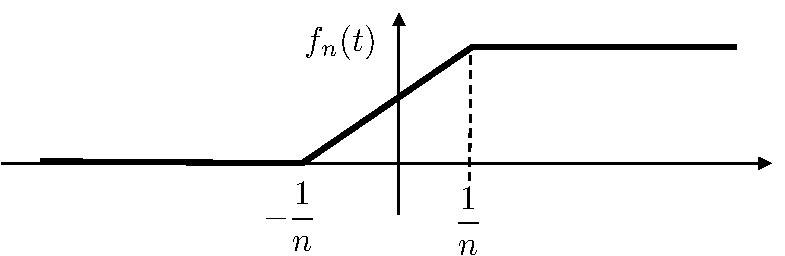
\includegraphics[width=0.6\textwidth]{figures/chap2_discontinuous_function}\\
\end{center}

By integration we get:
\[ d(f_n,f_n) = \frac{1}{6m^3n}(m^3+4m^2n + mn^2 + 2n^3) \]
\[\to 0 \text{ for } n,m \text{ large } (m > n) \]
but $f_n$ converges to a discontinuous function which is not in $\mathbb{X}$.  This is undesirable.
\end{example}
\end{frame}

%----------------------------------
\begin{frame}\frametitle{Topology: Complete Metric Space}

\begin{definition}[Complete metric space]
A metric space $(\mathbb{X},d)$ is \underline{complete} if every Cauchy sequence in $\mathbb{X}$ converges to a value in $\mathbb{X}$.\\
\end{definition}

\begin{block}{Implication}
 $C[a,b]$ with metric $(\int_{a}^{b}\abs{f-g}^2 dt)^{1/2}$ is \underline{not} complete.	
\end{block}

\begin{itemize}
\item Banach spaces are \underline{complete} normed spaces (discussed later).
\item Hilbert spaces (extremely important in signal processing and control) are complete inner product spaces (discussed later).
\item The importance of $L_p$ and $\ell_p$ are that they are complete spaces.
\end{itemize}

%$\rightarrow$ Notes on $L_p$:\\
%
%\quad $x \in L_p$ is actually a family of functions not a single function.  The following functions are equivalent:\\
%\includegraphics[width=0.9\textwidth]{chap2imgs/1-page6}\\
%
%In fact equivalent functions can differ at a countable infinite number of points!\\
%
%Technically they can differ on a set of measure zero.  All functions with the same Lebesque integral are said to be equivalent.\\
\end{frame}


\end{document}